%%% Folie
\begin{frame}{Ausgangslage}
    Hier die Ausgangslage/Motivation für das Kapitel beschreiben ...

    % UNGEFÄHRE AUSSAGE
    %
    % Dieselben Architekturmuster, die im Kleinen dazu genutzt werden können, einen
    % Quellcode in unabhängige Komponenten zu zerlegen, können im Großen auch genutzt
    % werden, um die Gesamtarchitektur eines IoT-Setups zu definieren. So können über
    % einen zentral gehosteten Message Broker mehrere Devices ganz einfach untereinander
    % Daten austauschen oder mit einem Cloud-Backend kommunizieren. Das mit Abstand
    % häufigste Protokoll hierfür ist MQTT, das vielen Programmiersprachen einfach
    % eingesetzt werden kann. Dieses Kapitel soll daher die Grundprinzipien asynchroner
    % Kommunikation mit dem Publish/Subscribe-Pattern vertiefen und zeigen, wie diese%
    % durch MQTT umgesetzt werden. Dabei soll auch gezeigt werden, wie MQTT zusammen mit
    % Python im Kontext eines typischen IoT-Cloudszenarios genutzt werden kann, um mehrere
    % Devices in einem Cloud-Dashboard zu überwachen.
\end{frame}

%%% Folie
\begin{frame}{Lernziele}
    \begin{itemize}
        \item Vor- und Nachteile asynchroner Kommunikationsmuster erklären können
        \item Skalierbare und ausfallsichere IoT-Architekturen entwerfen können
        \item Besonderheiten von MQTT bzgl. Publish/Subscribe kennen
        \item MQTT-Clients in Python entwickeln können
        \item Den Raspberry Pi in Python mit der Adafruit IO Cloud verbinden können
        \item Dashboards zur Überwachung und Steuerung mit Adafruit realisieren können
        %\item Einfache Workflows z.B: mit IFTTT oder Zapier realisieren können
    \end{itemize}
\end{frame}


%-------------------------------------------------------------------------------
\section{Adafruit IO}
%-------------------------------------------------------------------------------

%%% Folie
\begin{frame}{Folie}
\cite{Adafruit MQTTFx Setup}

\end{frame}

\begin{frame}{Limits in der Freien Version}

  \begin{figure}[!htb]
  \hspace*{5mm}
        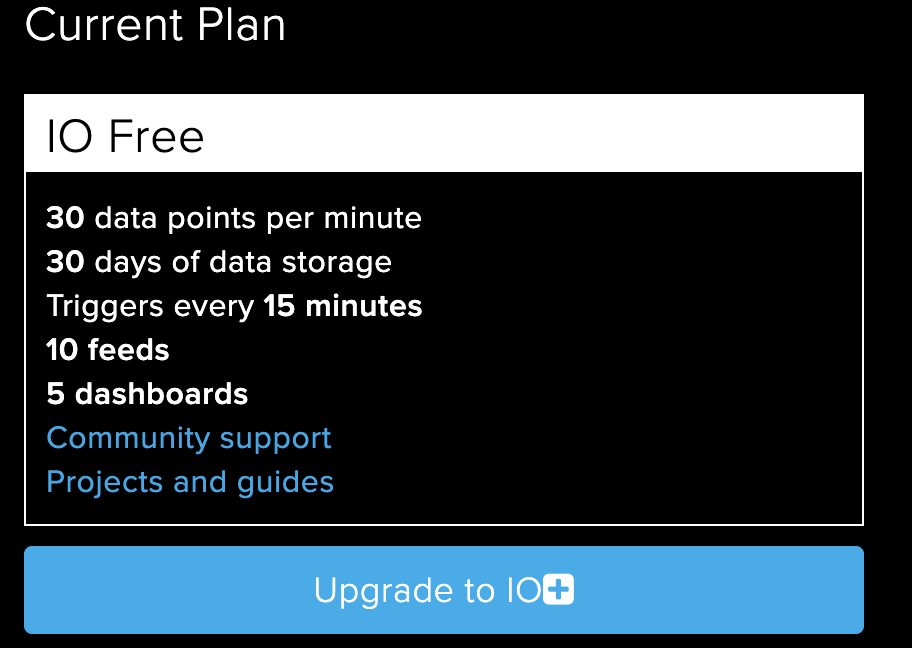
\includegraphics[scale=0.6]{7-datenaustausch/img/adafruit-limits} 
    \end{figure}
\end{frame}

%%% Folie
\begin{frame}{Unterschiede im Topic Handling}
    \begin{itemize}
        \setlength{\itemindent}{1.6in}
        \item [\textbf{Adafruit IO Besonderheiten}]
    \end{itemize}
    \begin{itemize}
        \item Statt der Topic Struktur aus MQTT werden im Adafruit IO sogenannte  \textbf{Feeds} verwendet \cite{io.adafruit.com/api/docs}
        \item Feeds sind \quotes{mehr als nur Topics}: Metadaten, Nachrichten, Lizenzinformation, Sichbarkeitskontrolle (private vs. public)
        \item Feeds können auch per REST API bedient werden:  \texttt{POST/api/v2/{username}/feeds} mit Inhalt z.B. Name/Beschreibung des Feeds
        \item In Adafruit gestalten sich Topics nach folgender Semantik: \texttt{userName/feeds/groupName.feedkey}
    \end{itemize}

    
\end{frame}

%%% Folie
\begin{frame}{Unterschiede bei Pub/Sub}
	\begin{figure}
	\centering
	\parbox{5cm}{
		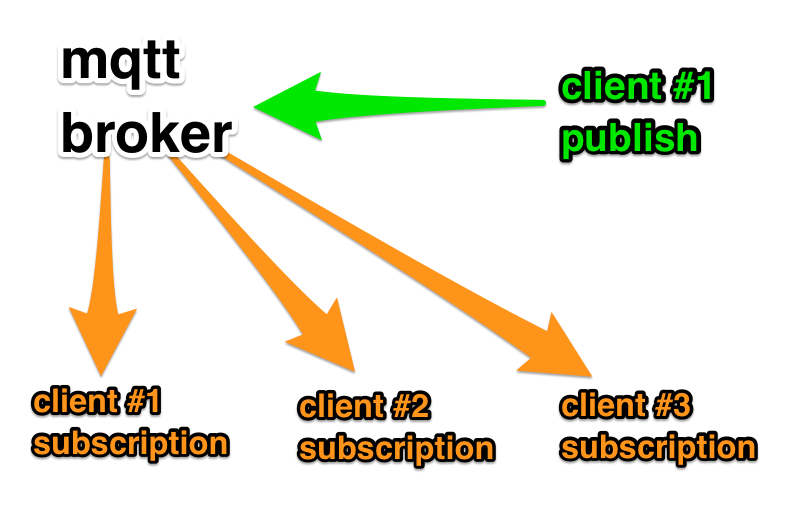
\includegraphics[scale=0.19]{7-datenaustausch/img/mqtt-pubsub}
		\caption{Pub/Sub in MQTT}
		\label{fig:pubsubmqtt}
		}
	\qquad
	\begin{minipage}{5cm}
		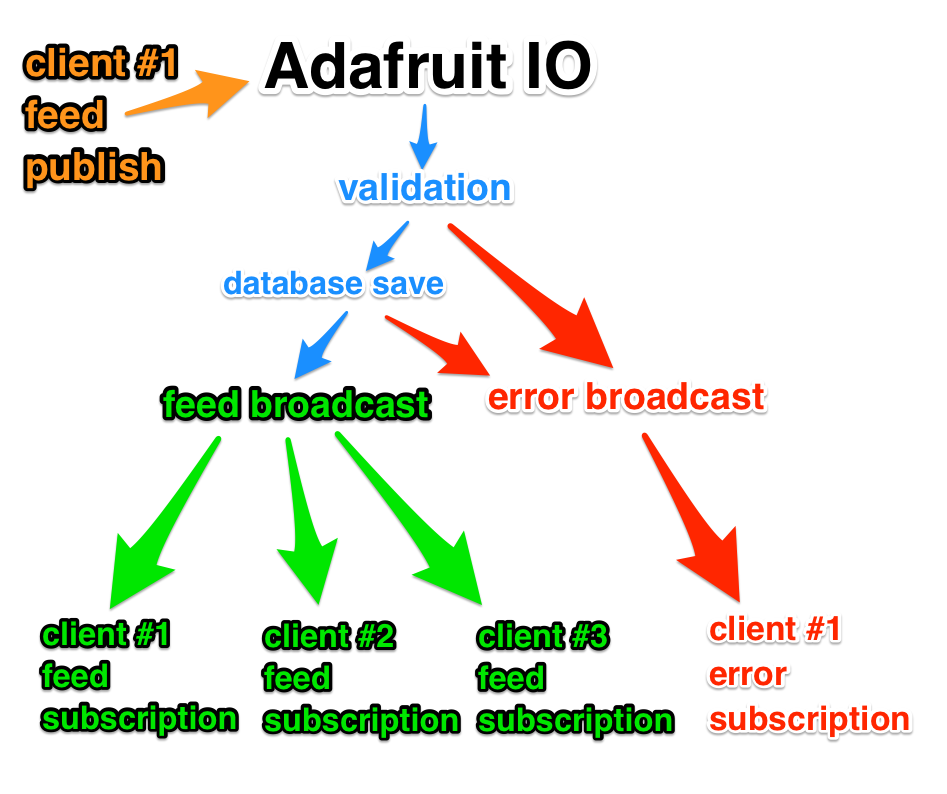
\includegraphics[scale=0.15]{7-datenaustausch/img/adafruit-pubsub}
		\caption{Pub/Sub in Adafruit}
		\label{fig:pubsubadafruit}
	\end{minipage}
\end{figure}


\end{frame}




%-------------------------------------------------------------------------------
\section{MQTT und das Internet of Things}
%-------------------------------------------------------------------------------

%%% Folie
\begin{frame}{Folie}
    TODO
\end{frame}

%%% Folie
\begin{frame}{Folie}
    TODO
\end{frame}

